
\section{HÀM SỐ MŨ, HÀM SỐ LOGARIT}
\subsection{Tóm tắt lý thuyết}
\begin{tomtat}
	\subsubsection{Hàm số mũ}
	\begin{dn}
		Cho số thực $a>0$ và khác $1$. Hàm số $y=a^x$ được gọi là hàm số mũ cơ số $a$.
	\end{dn}
	\begin{tc} Cho hàm số mũ $y=a^x$, trong đó $0<a \ne 1$.
		\begin{itemize}
			\item [$\bullet$] Tập xác định của hàm số $y=a^x$ là $\mathbb{R}$;
			\item [$\bullet$] Tập giá trị của hàm số $y=a^x$ là $(0;+\infty)$.
			\item Khi $a>1$ thì hàm số đồng biến trên $\mathbb{R}$.
			\item  Khi $0<a<1$ thì hàm số nghịch biến trên $\mathbb{R}$.
			\item Liên tục trên $\mathbb R$.
			\item  Đồ thị luôn qua $(0;1),(1;a)$ và luôn nằm phía trên trục hoành.
		\end{itemize}
		\hspace{1cm}
		\begin{center}
			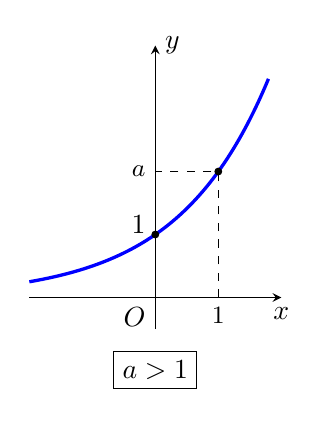
\begin{tikzpicture}[smooth,samples=300,scale=0.8,>=stealth]
			\draw[->] (-2,0)--(2,0) node[below]{$x$};
			\draw[->] (0,-0.5)--(0,4) node[right]{$y$};
			\draw (0,0) node[below left]{$O$};
			\draw[line width=1.2pt,color=blue,domain=-2:1.8] plot(\x,{2^(\x)});
			\draw[fill=black] (0,1) circle(1.5pt) (1,2) circle(1.5pt);
			\draw[dashed] (1,0)node[below]{\small $1$}--(1,2)--(0,2)node[left]{\small $a$};
			\node[below] at (0,-0.7) {\fbox{$a>1$}};
			\node[left] at (0,1.15) {$1$};
		\end{tikzpicture}
		\hspace{5cm}
		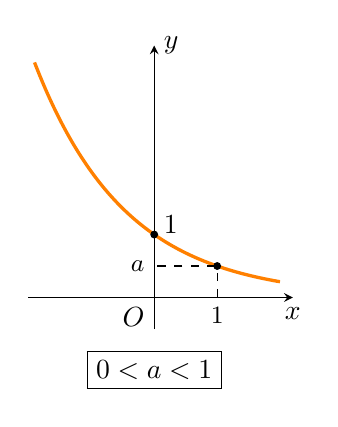
\begin{tikzpicture}[smooth,samples=300,scale=0.8,>=stealth]
			\draw[->] (-2,0)--(2.2,0) node[below]{$x$};
			\draw[->] (0,-0.5)--(0,4) node[right]{$y$};
			\draw (0,0) node[below left]{$O$};
			\draw[line width=1.2pt,color=orange,domain=-1.9:2] plot(\x,{0.5^(\x)});
			\draw[fill=black] (0,1) circle(1.5pt) (1,0.5) circle(1.5pt);
			%\draw[dashed] (-1,0)node[below]{\small $-1$}--(-1,2)--(0,2)node[right]{\small $\frac{1}{a}$};
			\draw[dashed] (1,0)node[below]{\small $1$}--(1,0.5)--(0,0.5)node[left]{\small $a$};
			\node[below] at (0,-0.7) {\fbox{$0<a<1$}};
			\node[right] at (0,1.15) {$1$};
		\end{tikzpicture}
		\end{center}
	\end{tc}
		\textbf{Ví dụ:} Vẽ đồ thị hàm số $y=\left( \dfrac{1}{2} \right)^{x}$.\\
		\textbf{Lời giải:} Lập bảng giá trị của hàm số tại một số điểm như sau:
			\begin{center}
				\begin{tabular}{|c|c|c|c|c|c|c|c|}
					\hline
					$ x $ & $-3$ & $-2$ & $-1$ & 0 & 1 & 2 & 3 \\
					\hline
					$y = \left( \dfrac{1}{2} \right)^{x}$ & 8 & 4 & 2 & 1 & $\dfrac{1}{2}$ & $\dfrac{1}{4}$ & $\dfrac{1}{8}$ \\
					\hline
				\end{tabular}
			\end{center}
			
			Từ đó, ta vẽ được đồ thị của hàm số $y=\left( \dfrac{1}{2} \right)^{x}$ như Hình 6.2.
			
			\begin{center}
				\begin{tikzpicture}[smooth,samples=300,scale=0.8,>=stealth]
					\draw[->] (-4,0)--(5,0) node[below]{$x$};
					\draw[->] (0,-1)--(0,9) node[right]{$y$};
					\draw (0,0) node[below left]{$O$};
					\draw[line width=1.2pt,color=red,domain=-3.1:4.5] plot(\x,{0.5^(\x)});
					\draw[fill=black] (0,1) circle(1pt) (0,2) circle(1pt) (0,3) circle(1pt) (0,4) circle(1pt) (0,5) circle(1pt) (0,6) circle(1pt) (0,7) circle(1pt) (0,8) circle(1pt) (-3,0) circle(1pt) (-2,0) circle(1pt) (-1,0) circle(1pt) (1,0) circle(1pt) (2,0) circle(1pt) (3,0) circle(1pt) (4,0) circle(1pt);
					\draw[dashed] (-3,0)node[below]{\small $-3$}--(-3,8)--(0,8)node[right]{\small $8$};
					\draw[dashed] (-2,0)node[below]{\small $-2$}--(-2,4)--(0,4)node[right]{\small $4$};
					\draw[dashed] (-1,0)node[below]{\small $-1$}--(-1,2)--(0,2)node[right]{\small $2$};
					\draw[dashed] (0,1/2)node[left]{\small $\frac{1}{2}$}--(1,1/2)--(1,0)node[below]{\small $1$};
					\draw[dashed] (0,1/4)--(2,1/4)--(2,0)node[below]{\small $2$};
					\draw[dashed] (0,1/8)--(3,1/8)--(3,0)node[below]{\small $3$};
					\node[right] at (0,1.15) {$1$};
					\node[below] at (0,-1.5) {$\text{Hình 6.2}$};
				\end{tikzpicture}
			\end{center}	
	\subsubsection{Hàm số logarit}
	\begin{dn}
		Cho số thực $a>0$ và khác $1$. Hàm số $y=\log_a x$ được gọi là hàm số logarit cơ số $a$.
	\end{dn}
	\begin{tc}
		Cho hàm số logarit $y=\log_ax$, trong đó $0<a \ne 1$.
		\begin{itemize}
			\item [$\bullet$] Tập xác định của hàm số $y=\log_ax$ là $(0;+\infty)$ ;
			\item [$\bullet$] Tập giá trị của hàm số $y=\log_ax$ là $\mathbb{R}$ .
			\item  Khi $a>1$ thì hàm số đồng biến trên $(0; +\infty)$ 
			\item  Khi $0<a<1$ thì hàm số nghịch biến trên $(0; +\infty)$ .
			\item Liên tục trên $(0;+\infty)$.
			\item  Đồ thị luôn qua $(1;0),(a;1)$ và luôn nằm bên phải trục tung.
		\end{itemize}
		\hspace{1cm}
		\begin{center}
			\begin{tikzpicture}[smooth,samples=300,scale=0.8,>=stealth]
			\draw[->] (-1,0)--(4,0) node[below]{$x$};
			\draw[->] (0,-2.5)--(0,2) node[right]{$y$};
			\draw (0,0) node[below left]{$O$};
			\draw[line width=0.8pt,color=violet,domain=0.2:3.2]plot(\x,{ln((\x))/ln(2)});
			\draw[fill=black] (1,0) circle(1.5pt) (2,1) circle(1.5pt);
			\draw[dashed] (2,0)node[below]{\small $a$}--(2,1)--(0,1)node[left]{\small $1$};
			\node[below] at (1,-2.6) {\fbox{$a>1$}};
			\node[below] at (1.1,0) {\small $1$};\end{tikzpicture}
		\hspace{5cm}
		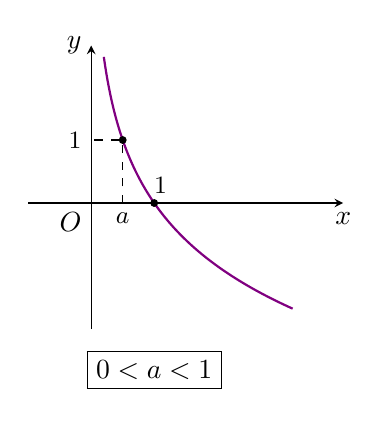
\begin{tikzpicture}[smooth,samples=300,scale=0.8,>=stealth]
			\draw[->] (-1,0)--(4,0) node[below]{$x$};
			\draw[->] (0,-2)--(0,2.5) node[left]{$y$};
			\draw (0,0) node[below left]{$O$};
			\draw[line width=0.8pt,color=violet,domain=0.2:3.2]plot(\x,{ln((\x))/ln(0.5)});
			\draw[fill=black] (1,0) circle(1.5pt) (0.5,1) circle(1.5pt);
			%\draw[dashed] (2,0)node[above]{\small $\dfrac{1}{a}$}--(2,-1)--(0,-1)node[left]{\small $-1$};
			\draw[dashed] (0.5,0)node[below]{\small $a$}--(0.5,1)--(0,1)node[left]{\small $1$};
			\node[below] at (1,-2.2) {\fbox{$0<a<1$}};
			\node[above] at (1.1,0) {\small $1$};
		\end{tikzpicture}
		\end{center}
	\end{tc}
	
	\textbf{Ví dụ:} Vẽ đồ thị hàm số $y= \log_{\tfrac{1}{2}} x$.\\
	\textbf{Lời giải:} Lập bảng giá trị của hàm số tại một số điểm như sau:
			\begin{center}
				\begin{tabular}{|c|c|c|c|c|c|c|c|}
					\hline
					$ x $ & $8$ & $4$ & $2$ & 1 & $\tfrac{1}{2}$ & $\tfrac{1}{4}$ & $\tfrac{1}{8}$ \\
					\hline
					$y = \log_{\tfrac{1}{2}} x$ & $-3$ & $-2$ & $-1$ & 0 & $1$ & $2$ & $3$ \\
					\hline
				\end{tabular}
			\end{center}
			
			Từ đó, ta vẽ được đồ thị của hàm số $y = \log_{\tfrac{1}{2}} x$ như Hình 6.4.
			
			\begin{center}
				\begin{tikzpicture}[smooth,samples=300,scale=0.8,>=stealth]
					\draw[->] (-1,0)--(9,0) node[below]{$x$};
					\draw[->] (0,-4)--(0,5) node[right]{$y$};
					\draw (0,0) node[below left]{$O$};
					\draw[line width=1.2pt,color=red,domain=0.05:8.5] plot(\x,{ln((\x))/ln(0.5)});
					\draw[fill=black] (0,1) circle(1pt) (0,2) circle(1pt) (0,3) circle(1pt) (0,4) circle(1pt) (0,-1) circle(1pt) (0,-2) circle(1pt) (0,-3) circle(1pt) (1,0) circle(1pt) (2,0) circle(1pt) (3,0) circle(1pt) (4,0) circle(1pt) (5,0) circle(1pt) (6,0) circle(1pt) (7,0) circle(1pt) (8,0) circle(1pt);
					\draw[dashed] (0,3)node[left]{\small $3$}--(1/8,3)--(1/8,0);
					\draw[dashed] (0,2)node[left]{\small $2$}--(1/4,2)--(1/4,0);
					\draw[dashed] (1/2,0)node[below]{\small $\frac{1}{2}$}--(1/2,1)--(0,1)node[left]{\small $1$};
					\draw[dashed] (2,0)node[above]{\small $2$}--(2,-1)--(0,-1)node[left]{\small $-1$};
					\draw[dashed] (4,0)node[above]{\small $4$}--(4,-2)--(0,-2)node[left]{\small $-2$};
					\draw[dashed] (8,0)node[above]{\small $8$}--(8,-3)--(0,-3)node[left]{\small $-3$};
					\draw (1,0)node[above]{\small $1$};
					\node[below] at (4.5,-4.5) {$\text{Hình 6.4}$};
				\end{tikzpicture}
			\end{center}	
	\subsubsection{Liên hệ đồ thị của hai hàm số}
	\immini{
		Đồ thị hàm số $y=a^x$ và $y=\log_ax$ đối xứng nhau qua đường phân giác của góc phần tư (đường thẳng $y=x$) thứ nhất.
	}{
		\hspace{1cm}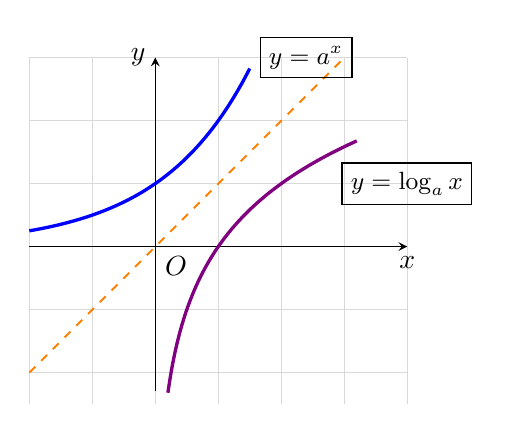
\begin{tikzpicture}[smooth,samples=300,scale=0.8,>=stealth]
			\draw [color=gray!30,, xstep=1.0cm,ystep=1.0cm] (-2,-2.5) grid (4,3);
			\draw[->] (-2,0)--(4,0) node[below]{$x$};
			\draw[->] (0,-2.3)--(0,3) node[left]{$y$};
			\draw (0,0) node[below right]{$O$};
			\draw[line width=1.2pt,color=blue,domain=-2:1.5] plot(\x,{2^(\x)});
			\draw[line width=1.2pt,color=violet,domain=0.2:3.2]plot(\x,{ln((\x))/ln(2)});
			\draw[dashed,line width=0.7pt,color=orange] (-2,-2)--(3,3);
			%\node[below] at (2,-1.2) {\small\fbox{Hình I.3}};
			\node[right] at (2.8,1) {\small\fbox{$y=\log_ax$}};
			\node[right] at (1.5,3) {\small\fbox{$y=a^x$}};
		\end{tikzpicture}
	}
\end{tomtat}
\begin{dang}{Bài toán thực tế liên môn}
	Một người gửi vào ngân hàng số tiền $A$ đồng, lãi suất $r$ mỗi tháng theo hình thức lãi kép, gửi theo phương thức không kì hạn. Tính số tiền cả vốn lẫn lãi mà người đó nhận được sau $N$ tháng?\\
	Phương pháp xây dựng công thức:\\
	Gọi $T_N$ là số tiền cả vốn lẫn lãi sau $N$ tháng. Ta có:\\
	\begin{itemize}
		\item Sau 1 tháng $(k=1): T_1=A+A \cdot r=A(1+r)$.
		\item Sau 2 tháng $(k=2): T_2=A(1+r)+A(1+r) \cdot r=A(1+r)^2$
		\item ...
		\item Sau $N$ tháng $(k=N): T_N=A(1+r)^N$
	\end{itemize}
	Vậy số tiền cả vốn lẫn lãi người đó có được sau $N$ tháng là:
	$$T_N=A(1+r)^N$$
\end{dang}
\subsubsection{Ví dụ minh hoạ}
\begin{vd}%[1K6BJ-4]
	Trong âm học, mức cường độ âm được tính bới công thức $L=10\log\left(\dfrac{I}{I_0}\right)$ (dB) (dB là đơn vị mức cường độ âm, đọc là đề-xi-ben), trong đó $I$ là cường độ âm tính theo W/m$^2$ và $I_0=10^{-12}$ W/m$^2$ là cường độ âm chuẩn (cường độ âm thấp nhất mà tai người bình thường có thể nghe được).
	\begin{center}
		(\textit{Nguồn:} Vật lí 12, NXB Giáo dục Việt Nam, năm 2017, trang 52,53)
	\end{center}
	\begin{enumerate}
		\item Mức cường độ âm $L$ thấp nhất mà tai người có thể nghe được là bao nhiêu?
		\item Cuộc trò chuyện có cường độ âm $10^{-9}$ W/m$^2$ thì có mức cường độ âm bằng bao nhiêu?
		\item Cường độ âm tại một khu văn phòng nằm trong miền từ $10^{-7}$ W/m$^2$ đến $5\cdot10^{-6}$ W/m$^2$ (tức là $10^{-7}\le I\le5\cdot10^{-6}$). Mức cường độ âm tại khu văn phòng này nằm trong khoảng nào? (Làm tròn kết quả đến hàng đơn vị).
	\end{enumerate}
	\loigiai{\begin{enumerate}
			\item Khi $I=I_0$ thì $L=10\log 1=0$ (dB). Vậy mức cường độ âm thấp nhất mà tai người bình thường có thể nghe được là $0$ (dB).
			\item Khi $I=10^{-9}$ W/m$^2$, ta có $L=10\log\dfrac{10^{-9}}{10^{-12}}=10\log10^3=30\log10=30$ (dB).
			\item Với $I=10^{-7}$ W/m$^2$, $L=10\log\dfrac{10^{-7}}{10^{-12}}=10\log10^5=50\log10=50$ (dB).\\
			Với $I=5\cdot10^{-6}$ W/m$^2$, $L=10\log\dfrac{5\cdot10^{-6}}{10^{-12}}=10\log\left(5\cdot10^6\right)=10(6+\log5)\approx67$ (dB).\\
			Hàm số $y=\log x$ đồng biến nên hàm số $y=10\log x$ cũng đồng biến.\\
			Do đó, từ $10^{-7}\le I\le5\cdot10^{-6}$ suy ra $50\le L\le67$.\\
			Vậy mức cường độ âm tại khu văn phòng nằm trong khoảng từ $50$ (dB) đến $67$ (dB).
	\end{enumerate}}
\end{vd}
\begin{vd}%[1K6BJ-4]
	Trong Vật lí, sự phân rã của các chất phóng xạ được cho bởi công thức: $m(t)=m_0 \cdot\left(\dfrac{1}{2}\right)^{\tfrac{t}{T}} ;$ trong đó $m_0$ là khối lượng chất phóng xạ ban đầu (tại thời điểm $t=0$ ), $m(t)$ là khối lượng chất phóng xạ tại thời điểm $t$ và $T$ là chu kì bán rã (Nguồn: Giải tích 12, NXBGD Việt Nam, 2021). Hạt nhân Poloni (Po) là chất phóng xạ $\alpha$ có chu kì bán rã là $138$ ngày (Nguồn: Vật lí 12, NXBGD Việt Nam, 2021). Giả sử lúc đầu có $100$ gam Poloni. Tính khối lượng Poloni còn lại sau $100$ ngày theo đơn vị gam (làm tròn kết quả đến hàng phần mười).
	\loigiai{
		Khối lượng Poloni còn lại sau $100$ ngày là
		$$m(100)=100 \cdot\left(\dfrac{1}{2}\right)^{\tfrac{100}{138}} \approx 60,5(\mathrm{~g}).$$}
\end{vd}
\begin{vd}%[1K6BJ-4]
	Lốc xoáy là hiện tượng một luồng không khí xoáy tròn mở rộng ra từ một đám mây dông xuống tới mặt đất. Các cơn lốc xoáy thường có sức tàn phá rất lớn. Tốc độ của gió (đơn vị: dặm/giờ) gần tâm của một cơn lốc xoáy được tính bởi công thức: $S=93 \log d+65$, (Nguồn: Ron Larson, Intermediate Algebra, Cengage) trong đó $d$ (đơn vị: dặm) là quãng đường cơn lốc xoáy di chuyển được. Hãy tính tốc độ của gió ở gần tâm (làm tròn kết quả đến hàng đơn vị) khi cơn lốc xoáy di chuyển được quãng đường là
	\begin{multicols}{2}
		\begin{enumerate}
			\item $5$ dặm
			\item $10$ dặm
		\end{enumerate}
	\end{multicols}
	\loigiai{
		\begin{enumerate}
			\item Tốc độ của gió ở gần tâm khi cơn lốc xoáy di chuyển được quãng đường $5$ dặm là
			$$S=93 \log 5+65 \approx 130 \text { (dặm/giờ).}$$
			\item Tốc độ của gió ở gần tâm khi cơn lốc xoáy di chuyển được quãng đường $10$ dặm là
			$$S=93 \log 10+65=158\text { (dặm/giờ)}.$$
		\end{enumerate}
	}
\end{vd}
\begin{vd}%[1K6BJ-4]
	Chỉ số hay độ pH của một dung dịch được tính theo công thức: $\mathrm{pH}=-\log \left[\mathrm{H}^{+}\right]$. Phân tích nồng độ ion hydrogen $\left[\mathrm{H}^{+}\right]$ trong hai mẫu nước sông, ta có kết quả sau: Mẫu 1: $\left[\mathrm{H}^{+}\right]=8 \cdot 10^{-7}$; Mẫu $2:\left[\mathrm{H}^{+}\right]=2 \cdot 10^{-9}$.
	Không dùng máy tính cầm tay, hãy so sánh độ pH của hai mẫu nước trên.
	\loigiai{
		Hàm số $\mathrm{pH}=-\log \left[\mathrm{H}^{+}\right]$ có $a=10>1$ nên nghịch biến trên $(0;+\infty)$.\\
		Vì $8 \cdot 10^{-7}>2 \cdot 10^{-9}$ nên độ pH của mẫu 1 bé hơn độ pH của mẫu 2.
	}
\end{vd}

\begin{vd}%[1K6BJ-4]
	Một người gửi $10$ triệu đồng vào ngân hàng theo hình thức lãi kép có kì hạn là 12 tháng vối lãi suất $6\%$/năm. Giả sử qua các năm thì lãi suất không thay đổi và người đó không gửi thêm tiền vào mỗi năm. Để biết sau $y$ (năm) thì tổng số tiền cả vốn và lãi có được là $x$ (đồng), người đó sử dụng công thức $y=\log_{1,06}\left(\dfrac{x}{10}\right)$. Hỏi sau bao nhiêu năm thì người đó có được tổng số tiền cả vốn và lãi là $15$ triệu đồng? $20$ triệu đồng? (Làm tròn kết quả đến hàng đơn vị).
	\loigiai{
		Người đó có được tổng số tiền cả vốn lẫn lãi là $15$ triệu đồng sau
		$$y=\log_{1,06}\left(\dfrac{15}{10}\right)\approx 7\text{ (năm).}$$
		Người đó có được tổng số tiền cả vốn lẫn lãi là $20$ triệu đồng sau
		$$y=\log_{1,06}\left(\dfrac{20}{10}\right)\approx 12\text{ (năm).}$$
	}
\end{vd}
\subsubsection{Bài tập}
\begin{bt}%[1K6YJ-4]
	Giả sử một chất phóng xạ bị phân rã theo cách sao cho khối lượng $m(t)$ của chất còn lại (tính bằng kilôgam) sau $t$ ngày được cho bởi hàm số $m(t) = 13 \mathrm{e}^{-0,0015t}$.
	\begin{enumerate}
		\item Tìm khối lượng của chất đó tại thời điểm $t = 0$.
		\item Sau 45 ngày khối lượng chất đó còn lại là bao nhiêu?
	\end{enumerate}
	\loigiai{
		\begin{enumerate}
			\item $m(0) = 13\mathrm e^{0} = 13$ (kilôgam).
			\item $m(45) = 13\mathrm e^{-0,015 \cdot  45} \approx 6{,}62$ (kilôgam).
		\end{enumerate}
	}
\end{bt}

\begin{bt}%[1K6YJ-4]
	Trong một nghiên cứu, một nhóm học sinh được cho xem cùng một danh sách các loài động vật và được kiểm tra lại xem họ còn nhớ bao nhiêu phần trăm danh sách đó sau mỗi tháng. Giả sử sau $t$ tháng, khả năng nhớ trung bình của nhóm học sinh đó được tính theo công thức $M(t) = 75 - 20 \ln (t+1), \enskip 0 \leq t \leq 12$ (đơn vị: \%). Hãy tính khả năng nhớ trung bình của nhóm học sinh đó sau 6 tháng.
	\loigiai{
		Khả năng nhớ trung bình của nhóm học sinh đó sau 6 tháng là $$M(6) = 75 - 20 \ln (6+1) \approx 36{,}1 \%.$$
	}
\end{bt}
\begin{bt}%[1K6BJ-4]
	Cường độ ánh sáng $I$ dưới mặt biển giảm dần theo độ sâu theo công thức $I=I_0\cdot a^d$, trong đó $I_0$ là cường độ ánh sáng tại mặt nước biển, $a>0$ là hằng số và $d$ là độ sâu tính bằng mét tính từ mặt nước biển.
	\begin{center}
		(\textit{Nguồn:}  http://www.britannica.com/science/seawer/Optical-properties)
	\end{center}
	\begin{enumerate}
		\item Có thể khẳng định rằng $0<a<1$ không? Giải thích.
		\item Biết rằng cường độ ánh sáng tại độ sâu $1$m bằng $0{,}95I_0$. Tìm giá trị của $a$.
		\item Tại độ sâu $20$m, cường độ ánh sáng bằng bao nhiêu phần trăm so với $I_0$? (Làm tròn kết quả đến hàng đơn vị.)
	\end{enumerate}
	\loigiai{\begin{enumerate}
			\item Do $I_0$ là cường độ ánh sáng tại mặt nước biển là không đổi, nên cường độ ánh sáng $I$ tỉ lệ thuận với hàm số $a^d$.\\
			Do $I$ giảm dần theo độ sâu, nên hàm số $a^d$ nghịch biến, suy ra $0<a<1$.
			\item Tại độ sâu $1$m, ta có cường độ ánh sáng $I=0{,}95I_0$, suy ra $0{,}95I_0=I_0a^1\Leftrightarrow a=0{,}95$.
			\item Tại độ sâu $20$m, suy ra $d=20$. Cường độ ánh sáng tại đó là $I=I_0a^d=I_0\cdot0{,}95^{20}\approx0{,}4I_0$.\\
			Vậy tại độ sâu $20$m, cường độ ánh sáng tại đó bằng khoảng $40$\% so với $I_0$.
	\end{enumerate}}
\end{bt}
\begin{bt}%[1K6BJ-4]
	Công thức $h=-19{,}4\cdot\log\dfrac{P}{P_0}$ là mô hình đơn giản cho phép tính độ cao $h$ so với mặt nước biển của một vị trí trong không trung (tính bằng ki-lô-mét) theo áp suất không khí $P$ tại điểm đó và áp suất $P_0$ của không khí tại mặt nước biển (cùng tính bằng $Pa$ - đơn vị áp suất, đọc là Pascal).
	\begin{center}
		(\textit{Nguồn:}  http://doi.org/10.1007/s40828-020-0111-6)
	\end{center}
	\begin{enumerate}
		\item Nếu áp suất không khí ngoài máy bay bằng $\dfrac{1}{2}P_0$ thì máy bay đang ở độ cao nào?
		\item Áp suất không khí tại đỉnh của ngọn núi A bằng $\dfrac{4}{5}$ lần áp suất không khí tại đỉnh của ngọn núi B. Ngọn núi nào cao hơn và cao hơn bao nhiêu ki-lô-mét? (Làm tròn kết quả đến hàng phần mười.)
	\end{enumerate}
	\loigiai{\begin{enumerate}
			\item Nếu áp suất ở ngoài máy bay là $\dfrac{1}{2}P_0$ thì độ cao của máy bay là $$h=-19{,}4\cdot\log\dfrac{\dfrac{1}{2}P_0}{P_0}=-19{,}4\cdot\log\dfrac{1}{2}\approx5{,}8\text{km}.$$
			\item Gọi áp suất lần lượt của hai ngọn núi A và B là $P_A$, $P_B$. Ta có $P_A=\dfrac{4}{5}P_B$.\\
			Độ cao của núi A và núi B là $\heva{&h_A=-19{,}4\cdot\log\dfrac{P_A}{P_0}\\&h_B=-19{,}4\cdot\log\dfrac{P_B}{P_0}.}$\\
			Ta có
			\begin{eqnarray*}
				h_A&=&-19{,}4\cdot\log\dfrac{P_A}{P_0}=-19{,}4\cdot\log\dfrac{\dfrac{4}{5}P_B}{P_0}\\
				&=&-19{,}4\cdot\left(\log\dfrac{4}{5}+\log\dfrac{P_B}{P_0}\right)=-19{,}4\cdot\log\dfrac{4}{5}+h_B\approx h_B+1{,}9.
			\end{eqnarray*}
			Vậy núi A cao hơn núi B $1{,}9$km.
	\end{enumerate}}
\end{bt}
\begin{bt}%[1K6BJ-4]
	Ta coi năm lấy làm mốc để tính dân số của một vùng (hoặc một quốc gia) là năm 0. Khi đó, dân số của quốc gia đó ở năm thứ $t$ là hàm số theo biến $t$ được cho bởi công thức: $S=A \cdot e^{rt}$. Trong đó $A$ là dân số của vùng (hoặc quốc gia) đó ở năm 0 và $r$ là tỉ lệ tăng dân số hằng năm (Nguồn: Giải tích 12, NXBGD Việt Nam, 2021). Biết rằng dân số Việt Nam năm 2021 ước tính là $98564407$ người và tỉ lệ tăng dân số $0,93\%$/năm (Nguồn: https://danso.org/viet-nam). Giả sử tỉ lệ tăng dân số hằng năm là như nhau tính từ năm 2021, nêu dự đoán dân số Việt Nam năm 2030 (làm tròn kết quả đến hàng đơn vị).
	\loigiai{
		Dân số Việt Nam vào năm 2030 là
		$$S=A \cdot e^{rt}=98564407\cdot e^{0,93\%\cdot 9}\approx 107169341\text{ (người).}$$
	}
\end{bt}

\begin{bt}%[1K6BJ-4]
	Các nhà tâm lí học sử dụng mô hình hàm số mũ để mô phỏng quá trình học tập của một học sinh như sau: $f(t)=c\left(1-e^{-k t}\right)$, trong đó $c$ là tổng số đơn vị kiến thức học sinh phải học, $k$ (kiến thức/ngày) là tốc độ tiếp thu của học sinh, $t$ (ngày) là thời gian học và $f(t)$ là số đơn vị kiến thức học sinh đã học được (Nguồn: R.I. Charles et al., Algebra 2, Pearson). Giả sử một em học sinh phải tiếp thu $25$ đơn vị kiến thức mới. Biết rằng tốc độ tiếp thu của em học $\sinh$ là $k=0{,}2$. Hỏi em học sinh sẽ nhớ được (khoảng) bao nhiêu đơn vị kiến thức mới sau $2$ ngày? Sau $8$ ngày?
	\loigiai{
		Số đơn vị kiến thức mới em học sinh sẽ nhớ sau $2$ ngày là
		$$f(2)=25\left(1-e^{-0{,}2\cdot2}\right)\approx 8{,}24\text{ (đơn vị)}.$$
		Số đơn vị kiến thức mới em học sinh sẽ nhớ sau $8$ ngày là
		$$f(8)=25\left(1-e^{-0{,}2\cdot8}\right)\approx 19{,}95\text{ (đơn vị)}.$$
	}	
\end{bt}
\subsubsection{Câu hỏi trắc nghiệm}
\Opensolutionfile{ans}[ans/ans-1K6-20-Dang4]
\begin{ex}%[1K6YJ-4]
	Số lượng của một loài vi khuẩn sau $t$ (giờ) được cho xấp xỉ bởi đẳng thức $Q(t)=Q_{0} \cdot \mathrm{e}^{0{,}195 t}$, trong đó $Q_{0}$ là số lượng vi khuấn ban đầu. Nếu số lượng vi khuẩn ban đầu là $5000$ con thì sau bao nhiêu giờ, số lượng vi khuẩn có $100\, 000$ con?
	\choice
	{$20$ giờ}
	{$24$ giờ}
	{\True $15{,}36$ giờ}
	{$3{,}55$ giờ}
	\loigiai{
		Ta có $100\, 000 = 5000 \cdot \mathrm{e}^{0{,}195 t} \Leftrightarrow t= \dfrac{\ln 20}{0{,}195} \approx 15{,}36$ (giờ).
	}
\end{ex}

\begin{ex}%[1K6YJ-4]
	Một người gửi 75 triệu đồng vào ngân hàng theo thể thức lãi kép kì hạn 1 năm với lãi suất
	$5,4\%$/năm. Giả sử lãi suất không thay đổi, hỏi sau 6 năm thì người đó nhận về số tiền là bao nhiêu kể cả gốc và lãi? (làm tròn đến nghìn đồng).
	\choice
	{\True $102.826.000$ đồng}
	{$97.860.000$ đồng}
	{$150.260.000$ đồng}
	{$120.628.000$ đồng}
	
	\loigiai{Số tiền thu được sau 6 năm là $C= 75(1+0.054)^6=102.826.470$ đồng. }
	
\end{ex}

\begin{ex}%[1K6YJ-4]
	Một người gửi vào ngân hàng $500$ triệu đồng với lãi suất $0{,}6\%$ một tháng, sau mỗi tháng lãi suất được nhập vào vốn. Hỏi sau một năm người đó rút tiền thì tổng số tiền người đó nhận được là bao nhiêu?
	\choice
	{$500 \cdot 1{,}006$ (triệu đồng)}
	{$500 \cdot 1{,}06^{12}$ (triệu đồng)}
	{$500 \cdot (1+12\cdot 0{,}006)^{12}$ (triệu đồng)}
	{\True $500 \cdot 1{,}006^{12}$ (triệu đồng)}
	\loigiai{
		Công thức lãi suất $A(1+x\%)^n = 500\cdot(1+0{,}6\%)^{12} = 500 \cdot 1{,}006^{12}$.
	}
\end{ex}

\begin{ex}%[1K6YJ-4]
	Giả sử cứ sau một năm diện tích rừng của nước ta giảm $x$ phần trăm diện tích hiện có. Hỏi sau đây 4 năm diện tích rừng của nước ta sẽ là bao nhiêu phần trăm diện tích hiện nay?
	\choice
	{ $(1-x)^4$}
	{$1-\dfrac{4x}{100}$}
	{$1-\left(\dfrac{x}{100}\right)^4$}
	{\True $\left(1-\dfrac{x}{100}\right)^4$}
	\loigiai{
		Diện tích rừng lúc đầu là $S$, diện tích rừng sau 4 năm là $S_0$; $x \%=\dfrac{x}{100}$. Ta có
		$$S=S_0\left(1-\dfrac{x}{100}\right)^n=S_0\left(1-\dfrac{x}{100}\right)^4 \Leftrightarrow\dfrac{S}{S_0}=\left(1-\dfrac{x}{100}\right)^4.$$
	}
\end{ex}

\begin{ex}%[1K6BJ-4]
	Ông $V$ gửi tiết kiệm $200$ triệu đồng vào ngân hàng với hình thức lãi kép và lãi suất $7{,}2\%$ một năm. Hỏi sau $5$ năm ông $V$ thu về số tiền (cả vốn lẫn lãi) gần nhất với số nào sau đây?
	\choice
	{$283.145.000$ đồng}
	{$283.155.000$ đồng}
	{\True $283.142.000$ đồng}
	{$283.151.000$ đồng}
	\loigiai
	{Gọi $T$ là tổng số tiền thu được sau $5$ năm. \\
		Khi đó $T=200.000.000\left(1+\dfrac{7{,}2}{100}\right)^5 \approx 283.142.000$ đồng.}
\end{ex}

\begin{ex}%[1K6BJ-4]%[Phát triển đề Minh Họa 2020 - Lý Văn Hoàng]% Câu 25.1
	Biết rằng tỉ lệ tăng dân số thế giới hàng năm là $1{,}32\%$, nếu tỉ lệ tăng dân số không thay đổi thì dân số được tính theo công thức tăng trưởng liên tục $S=A\cdot \mathrm{e}^{Nr}$, trong đó $A$ là dân số tại thời điểm mốc, $S$ là số dân sau $N$ năm, $r$ là tỉ lệ tăng dân số hằng năm. Năm $2013$ dân số thế giới vào khoảng $7095$ triệu người. Hỏi  năm $2020$ dân số thế giới gần nhất với giá trị nào sau đây?
	\choice
	{$7879$ triệu người}
	{$7680$ triệu người}
	{\True $7782$ triệu người}
	{$7777$ triệu người}
	\loigiai{
		Theo giả thiết ta được $A= 7095$, $r= 1{,}32\%$, $N=2020-2013=7$.\\
		Áp dụng công thức $S=A\cdot \mathrm{e}^{Nr}$ ta được dân số thế giới năm $2020$  là\\
		\centerline{$S= 7095 \cdot {\mathrm{e}}^{7\cdot \frac{1{,}32}{100}} \approx 7781{,}82$ triệu người.}
	}
\end{ex}

\begin{ex}%[1K6BJ-4]
	Cường độ ánh sáng đi qua môi trường nước biển giảm dần theo công thức $I=I_0\cdot \mathrm{e}^{-\mu x}$, với $I_0$ là cường độ ánh sáng bắt đầu đi vào môi trường nước biển và $x$ là độ dày của môi trường đó ($x$ tính theo đơn vị mét). Biết rằng môi trường nước biển có hằng số hấp thụ là $\mu =1{,}4$. Hỏi ở độ sâu $30$ mét thì cường độ ánh sáng giảm đi bao nhiêu lần so với cường độ ánh sáng lúc ánh sáng bắt đầu đi vào nước biển?
	\choice
	{$\mathrm{e}^{-21}$ lần}
	{\True $\mathrm{e}^{42}$ lần}
	{$\mathrm{e}^{21}$ lần}
	{$\mathrm{e}^{-42}$ lần}
	\loigiai{
		Cường độ ánh sáng lúc bắt đầu đi vào nước biển là $I_0$.\\
		Ở độ sâu $x=30$ mét với hằng số hấp thụ là $\mu =1{,}4$, cường độ ánh sáng đi vào nước biển là
		$$I=I_0\cdot \mathrm{e}^{-\mu x}=I_0\cdot \mathrm{e}^{-30\cdot 1{,}4}=I_0\cdot \mathrm{e}^{-42}=\dfrac{I_0}{\mathrm{e}^{42}}.$$
		Vậy ở độ sâu $30$ mét thì cường độ ánh sáng giảm đi $\mathrm{e}^{42}$ lần so với cường độ ánh sáng lúc ánh sáng bắt đầu đi vào nước biển.
	}
\end{ex}

\begin{ex}%[1K6KJ-4]
	Gọi $I(t)$ là số ca bị nhiễm bệnh Covid-19 ở quốc gia X sau $t$ ngày khảo sát. Khi đó ta có công thức $I(t)=A\cdot\mathrm{e}^{r_0(t-1)}$ với $A$ là số ca bị nhiễm trong ngày khảo sát đầu tiên, $r_0$ là hệ số lây nhiễm. Biết rằng ngày đầu tiên khảo sát có $500$ ca bị nhiễm bệnh và ngày thứ $10$ khảo sát có $1000$ ca bị nhiễm bệnh. Hỏi ngày thứ $15$ số ca nhiễm bệnh gần nhất với số nào dưới đây, biết rằng trong suốt quá trình khảo sát hệ số lây nhiễm là không đổi?
	\choice
	{$1740$}
	{$2020$}
	{\True $1470$}
	{$1320$}
	\loigiai{Từ giả thiết ta có $\heva{&I(1)=500\\&I(10)=1000}\Leftrightarrow\heva{&A=500\\&A\cdot\mathrm{e}^{9r_0}=1000}\Leftrightarrow\heva{&A=500\\&r_0=\dfrac{1}{9}\ln 2.}$\\
		Số ca nhiễm bệnh ở ngày thứ $15$ là $I(15)=A\cdot\mathrm{e}^{14r_0}=500\cdot\mathrm{e}^{14\cdot\tfrac{1}{9}\ln 2}\approx1469{,}73\approx1470$.}
\end{ex}

\begin{ex}%[1K6KJ-4]
	Sự tăng trưởng của một loài vi khuẩn tuân theo công thức $N=A.e^{rt}$ trong đó $A$ là số lượng vi khuẩn ban đầu, $r$ là tỉ lệ tăng trưởng ($r>0$) và $t$ là thời gian tăng trưởng. Biết số lượng vi khuẩn ban đầu có $250$ con và sau $12$ giờ là $1500$ con. Hỏi sau bao lâu thì số lượng vi khuẩn tăng gấp $216$ lần số lượng vi khuẩn ban đầu?
	\choice
	{$66$ giờ}
	{$48$ giờ}
	{\True $36$ giờ}
	{$24$ giờ}
	\loigiai{
		Theo công thức ta có $1500=250\cdot e^{12r}\Leftrightarrow e^{12r}=6 \Leftrightarrow r=\dfrac{1}{12}\cdot \ln 6$.\\
		Khi đó $54000=250\cdot e^{\frac{t}{12}\ln 6}\Leftrightarrow 6^{\frac{t}{12}}=216\Leftrightarrow \dfrac{t}{12}=\log_6 216 =3 \Leftrightarrow t=36$ giờ.
	}
\end{ex}

\begin{ex}%[1K6GJ-4]
	Ngày $20/5/2019$, ngày con trai đầu lòng chào đời, chú Tuấn quyết định mở một tài khoản tiết kiệm ở ngân hàng cho con với lãi suất $0,5\%$/tháng. Kể từ đó, cứ vào ngày 21 hàng tháng, chú sẽ gửi vào tài khoản một triệu đồng. Sau mỗi tháng, số tiền lãi sẽ được nhập vào vốn ban đầu để tính lãi cho tháng tiếp theo. Hỏi vào ngày $22/5/2037$, số tiền trong khoản tiết kiệm đó là bao nhiêu? (làm tròn đến triệu đồng)
	\choice
	{$388$ triệu đồng}
	{$391$ triệu đồng}
	{$387$ triệu đồng}
	{\True $390$ triệu đồng}
	\loigiai{
		Gọi $T$ là số tiền gửi vào hàng tháng, $T_n$ là số tiền sau tháng $n$ kể từ ngày gửi lần đầu.\\
		Sau $1$ tháng, số tiền trong tài khoảng là $T_1=T+T\cdot r=T(1+r)$.\\
		Sau $2$ tháng, số tiền trong tài khoảng là $T_2=T\left[(1+r)^2+(1+r)\right]$.\\
		Sau $3$ tháng, số tiền trong tài khoảng là $T_3=T\left[(1+r)^3+(1+r)^2+(1+r)\right]$.\\
		\ldots \\
		Cứ như vậy, số tiền trong tài khoản sau $n$ tháng là $$T_n=T\left[(1+r)^n+(1+r)^{n-1}+\cdots+(1+r)\right]=T(1+r)\cdot \dfrac{(1+r)^n-1}{r}.$$
		Số tiền trong khoản tiết kiệm vào ngày $22/5/2036$ (sau $216$ tháng) là:
		$S=T_{216} + T=390$ triệu đồng.
	}
\end{ex}
\Closesolutionfile{ans}
% % \indapan{10}{ans}

